\documentclass[a4paper,12pt,oneside]{scrbook}

\usepackage[onehalfspacing]{setspace}

% TODO: Indentación del primer parrafo
% TODO: Imagenes vectoriales: https://creativecommons.org/mission/downloads/
% TODO: Título mas parecido al original

\usepackage{fontspec}
\usepackage{amsmath}
\usepackage{unicode-math}   % Incluye Latin Modern Math

\setmainfont[Ligatures=TeX]{Latin Modern Sans}
\setsansfont[Ligatures=TeX]{Latin Modern Sans}
\setmonofont[Scale=MatchLowercase]{Inconsolata}
\setmathfont{Latin Modern Math}

\recalctypearea

\usepackage[spanish,es-ucroman,es-noenumerate,es-tabla]{babel}

\usepackage[ruled,vlined,commentsnumbered,linesnumbered,inoutnumbered,titlenotnumbered,noend]{algorithm2e}
\SetKwRepeat{Do}{do}{while}

%\usepackage{alltt}
%\usepackage{multirow}
%\usepackage{array} 
%\usepackage{bigstrut}
%\usepackage{booktabs}
\usepackage{caption}
%\usepackage{enumitem,lipsum}
\usepackage{float}
%\usepackage{microtype}
\usepackage{graphicx}
\usepackage[hidelinks]{hyperref}
\usepackage{natbib}
\usepackage{pdflscape}
\usepackage{rotating}
\usepackage{subcaption}
%\usepackage{ctable}
%\usepackage{enumerate}
%\usepackage{gensymb}
%\usepackage{eurosym}
\usepackage{tabu}

%\usepackage{lineno}
%\\linenumbers
%\setlength\linenumbersep{5pt}
%\renewcommand\linenumberfont{\normalfont\tiny\sffamily\color{gray}}

\newenvironment{sourcecode}
{\begin{list}{}{\setlength{\leftmargin}{1em}}\item\scriptsize\bfseries}
{\end{list}}

\newenvironment{littlesourcecode}
{\begin{list}{}{\setlength{\leftmargin}{1em}}\item\tiny\bfseries}
{\end{list}}

\newenvironment{abstract}
{\par\noindent\begin{center}\textbf{\abstractname}\end{center}\begin{itshape}\par\noindent}
{\end{itshape}}

\newenvironment{summary}
{\par\noindent\begin{center}\textbf{Abstract}\end{center}\begin{itshape}\par\noindent}
{\end{itshape}}

\newenvironment{keywords}
{\begin{list}{}{\setlength{\leftmargin}{1em}}\item[\hskip\labelsep \bfseries Keywords:]}
{\end{list}}

\newenvironment{palabrasClave}
{\begin{list}{}{\setlength{\leftmargin}{1em}}\item[\hskip\labelsep \bfseries Palabras clave:]}
{\end{list}}

\usepackage{listings}
\usepackage{xcolor}

\colorlet{punct}{red!60!black}
\definecolor{background}{HTML}{EEEEEE}
\definecolor{delim}{RGB}{20,105,176}
\colorlet{numb}{magenta!60!black}

\lstdefinelanguage{json}{
    basicstyle=\normalfont\ttfamily,
    numbers=left,
    numberstyle=\scriptsize,
    stepnumber=1,
    numbersep=8pt,
    showstringspaces=false,
    breaklines=true,
    frame=lines,
    backgroundcolor=\color{background},
    literate=
     *{0}{{{\color{numb}0}}}{1}
      {1}{{{\color{numb}1}}}{1}
      {2}{{{\color{numb}2}}}{1}
      {3}{{{\color{numb}3}}}{1}
      {4}{{{\color{numb}4}}}{1}
      {5}{{{\color{numb}5}}}{1}
      {6}{{{\color{numb}6}}}{1}
      {7}{{{\color{numb}7}}}{1}
      {8}{{{\color{numb}8}}}{1}
      {9}{{{\color{numb}9}}}{1}
      {:}{{{\color{punct}{:}}}}{1}
      {,}{{{\color{punct}{,}}}}{1}
      {\{}{{{\color{delim}{\{}}}}{1}
      {\}}{{{\color{delim}{\}}}}}{1}
      {[}{{{\color{delim}{[}}}}{1}
      {]}{{{\color{delim}{]}}}}{1},
}

\renewcommand\chapterlinesformat[3]{\Ifstr{#2}{}{}{#2\\*\vspace{20pt}}\LARGE#3}
\renewcommand{\chapterformat}{%
  \chapapp~\thechapter%
}

\renewcommand\listtablename{Índice de Tablas}    
\renewcommand\listfigurename{Índice de Figuras} 

\begin{document}   

%%%%%%%%%%%%%%%%%%%%%%%%%%%%%%%%%%%%%%%%%%%%%%%%%%%%%%%%%%%%%%%%%%%%%%%%%%%%%%%
% First Page
%%%%%%%%%%%%%%%%%%%%%%%%%%%%%%%%%%%%%%%%%%%%%%%%%%%%%%%%%%%%%%%%%%%%%%%%%%%%%%%
\pagestyle{empty}

\newcommand{\HRule}{\rule{\linewidth}{1mm}}
\setlength{\parindent}{0mm}
\setlength{\parskip}{0mm}

\vspace*{\stretch{0.5}}

\begin{center}

\includegraphics[scale=0.8]{images/escuela-ingenieria-tecnologia-original}\\[10mm]
{\Huge Trabajo de Fin de Grado}
\end{center}

\HRule
\begin{flushright}
        {\Huge Título del trabajo} \\[2.5mm]
        {\Large \textit{Título del trabajo en inglés}} \\[5mm]
        {\Large Nombre y apellidos} \\[5mm]


\end{flushright}
\HRule
\vspace*{\stretch{2}}
\begin{center}
  \Large La Laguna, \today
\end{center}

\setlength{\parindent}{5mm}

%%%%%%%%%%%%%%%%%%%%%%%%%%%%%%%%%%%%%%%%%%%%%%%%%%%%%%%%%%
% Signature page (add the official stamp)
%%%%%%%%%%%%%%%%%%%%%%%%%%%%%%%%%%%%%%%%%%%%%%%%%%%%%%%%%%
\frontmatter
\cleardoublepageusingstyle{empty}
\thispagestyle{empty}

D. \textbf{Nombre Apellido1 Apellido2}, profesor Titular de Universidad adscrito al Departamento de Nombre del Departamento de la Universidad de La Laguna, como tutor

\bigskip
D. \textbf{Nombre Apellido1 Apellido2}, profesor Titular de Universidad adscrito al Departamento de Nombre del Departamento de la Universidad de La Laguna, como cotutor\pagestyle{empty}

\bigskip
\bigskip
\textbf{C E R T I F I C A (N)}

\bigskip
\bigskip
Que la presente memoria titulada:

\bigskip
''\textit{Título del Trabajo}''

\bigskip
\bigskip
\bigskip

\noindent ha sido realizada bajo su dirección por D. \textbf{Nombre Apellido1 Apellido2}.

\bigskip
\bigskip

Y para que así conste, en cumplimiento de la legislación vigente y a los efectos
oportunos, firman la presente en La Laguna a \today

%%%%%%%%%%%%%%%%%%%%%%%%%%%%%%%%%%%%%%%%%%%%%%%%%%%%%%%%%%
\cleardoublepageusingstyle{empty}
\thispagestyle{empty}

{ \flushright

\begin{LARGE}
Agradecimientos
\end{LARGE}

\hspace{3mm}

\begin{large}
XXX
XXX
XXX
XXX
\end{large}

}
%%%%%%%%%%%%%%%%%%%%%%%%%%%%%%%%%%%%%%%%%%%%%%%%%%%%%%%%
\newpage
\cleardoublepageusingstyle{empty}
\thispagestyle{empty}

\bigskip
\begin{LARGE}
Licencia
\end{LARGE}

\bigskip
* Si NO quiere permitir que se compartan las adaptaciones de tu obra y NO quieres permitir usos comerciales de tu obra, indica:

\begin{center}

\includegraphics[scale=1.8]{images/by-nc-nd_88x31}\\[5mm]
\end{center}

\begin{large}
© Esta obra está bajo una licencia de Creative Commons Reconocimiento-NoComercial-SinObraDerivada 4.0 Internacional.
\end{large}

\bigskip
\bigskip
\bigskip
* Si quiere permitir que se compartan las adaptaciones de tu obra mientras se comparta de la misma manera y NO quieres permitir usos comerciales de tu obra, indica:

\begin{center}

\includegraphics[scale=1.8]{images/by-nc-sa_88x31}\\[5mm]
\end{center}

\begin{large}
© Esta obra está bajo una licencia de Creative Commons Reconocimiento-NoComercial-CompartirIgual 4.0 Internacional.
\end{large}

\bigskip
\bigskip
\bigskip
* Si quiere permitir que se compartan las adaptaciones de tu obra y NO quieres permitir usos comerciales de tu obra, indica:

\begin{center}

\includegraphics[scale=1.8]{images/by-nc_88x31}\\[5mm]
\end{center}

\begin{large}
© Esta obra está bajo una licencia de Creative Commons Reconocimiento-NoComercial 4.0 Internacional.
\end{large}

\bigskip
\bigskip
\bigskip
*Si NO quiere permitir que se compartan las adaptaciones de tu obra y quieres permitir usos comerciales de tu obra, indica:

\begin{center}

\includegraphics[scale=1.8]{images/by-nd_88x31}\\[5mm]
\end{center}

\begin{large}
© Esta obra está bajo una licencia de Creative Commons Reconocimiento-SinObraDerivada 4.0 Internacional.
\end{large}

\bigskip
\bigskip
\bigskip
* Si quiere permitir que se compartan las adaptaciones de tu obra mientras se comparta de la misma manera y quieres permitir usos comerciales de tu obra (licencia de Cultura Libre) indica:

\begin{center}

\includegraphics[scale=1.8]{images/by-sa_88x31}\\[5mm]
\end{center}

\begin{large}
© Esta obra está bajo una licencia de Creative Commons Reconocimiento-CompartirIgual 4.0 Internacional.
\end{large}

\bigskip
\bigskip
\bigskip
* Si quiere permitir que se compartan las adaptaciones de tu obra y quieres permitir usos comerciales de tu obra (licencia de Cultura Libre) indica:

\begin{center}

\includegraphics[scale=1.8]{images/by_88x31}\\[5mm]
\end{center}

\begin{large}
© Esta obra está bajo una licencia de Creative Commons Reconocimiento 4.0 Internacional.
\end{large}

%%%%%%%%%%%%%%%%%%%%%%%%%%%%%%%%%%%%%%%%%%%%%%%%%%%%%%%%
\cleardoublepageusingstyle{empty}
\thispagestyle{empty}
\vspace*{200px}

\begin{abstract}
{\em
xxxxx
}

\begin{palabrasClave}
xxxxx, xxxx, xxxx
\end{palabrasClave}

\end{abstract}
%%%%%%%%%%%%%%%%%%%%%%%%%%%%%%%%%%%%%%%%%%%%%%%%%%%%%%%%%
\cleardoublepageusingstyle{empty}
\thispagestyle{empty}
\vspace*{200px}

\begin{summary}
{
xxxxx
}

\begin {keywords}
xxxx, xxxx, xxxx
\end {keywords}

\end{summary}

%%%%%%%%%%%%%%%%%%%%%%%%%%%%%%%%%%%%%%%%%%%%%%%%%%%%%%%%%
\cleardoublepage
\setcounter{page}{1} 

\tableofcontents
\listoffigures
\listoftables

\mainmatter

%%%%%%%%%%%%%%%%%%%%%%%%%%%%%%%%%%%%%%%%%%%%%%%%%%%%%%%%%%%%%%%%%%%%%%%%%%%%%%%
\chapter{Introducción}
\label{chapter:intro}

\chapter{Introducción}
\label{ch:intro}

\noindent Cualquier capítulo puede tener múltiples apartados, como el \autoref{sec:apartado1} o el \autoref{sec:sección2} de este mismo capítulo.

También está el \autoref{sec:ch2_1} del \autoref{ch:dos} que tiene la \autoref{fig:other}.

Es buena idea usar \verb|\noindent| al principio del primer párrafo, tras el encabezado de una sección o capítulo, para desactivar la sangría temporalmente.

\section{Listas de elementos}
\label{sec:apartado1}

\noindent Esta la lista de elementos del \autoref{sec:apartado1}:

\begin{itemize}
    \item Item 1
    \begin{itemize}
        \item Item 1
        \item Item 2
        \item Item 3
        \item Item 4
    \end{itemize}
    
    \item Item 2
    \item Item 3
    \item Item 4
\end{itemize}

\section{Enumeraciones}
\label{sec:sección2}

\noindent Esto es una lista enumerada, que puede estar relacionada con la \autoref{fig:intro}

\begin{enumerate}
    \item Item 1
    \begin{enumerate}
        \item Item 1
        \item Item 2
        \item Item 3
    \end{enumerate}
    \item Item 2
    \item Item 3
\end{enumerate}

\section{Figuras y tablas}

\noindent En la \autoref{fig:intro} se puede ver una figura de ejemplo. Las tablas, las figuras y los algoritmos (ver el \autoref{Apendice1:ZZZ}) son flotantes. Esto quiere decir que \LaTeX{} los intentará ubicar en el mejor lugar posible al componer el documento, intentando respetar ciertas reglas tipográficas. Como este lugar puede ser diferente a la posición que realmente ocupan en el texto, \textbf{es importante referenciar en el texto todas las figuras y las tablas}, en los diferentes puntos donde se hable de ellas.

\begin{figure}[htbp]
   \centering
   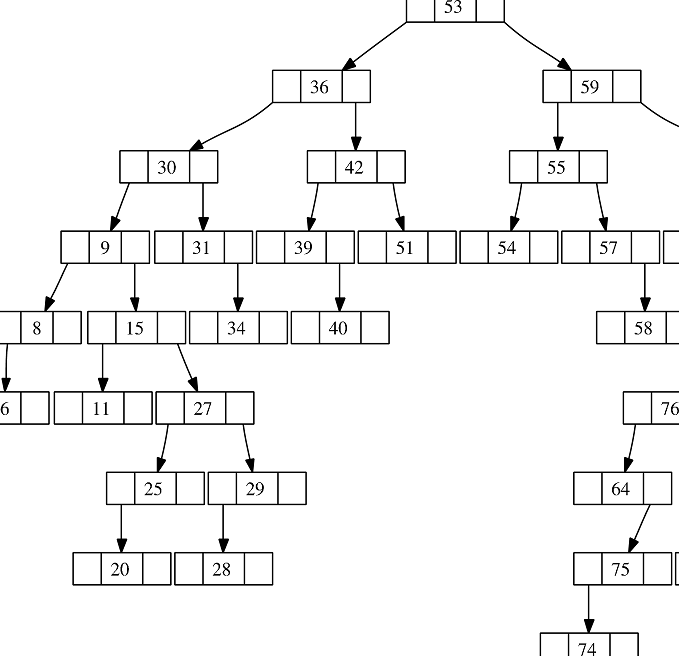
\includegraphics[width=0.8\linewidth]{images/figura_1}
   \caption{Ejemplo de figura.}
   \label{fig:intro}
\end{figure}

La \autoref{tbl:presupuesto} en el \autoref{ch:presupuesto} es un ejemplo de tabla hecha con el paquete \verb|tabularx|.

Al crear tablas, figuras u otros elementos flotantes es aconsejable indicar siempre los especificadores de ubicación \verb|[htbp]|, tal y como se hace en los ejemplos de esta plantilla. De esta forma \LaTeX{} intentará primero ponerlos en el lugar; si no puede, intentará ponerlos en la parte superior o inferior de la misma página y, en caso extremo, los pondrá en páginas especiales que solo contienen flotantes.

No es buena idea usar especificadores como \verb|[!h]| o \verb|[H]| para forzar una ubicación determinada. El motivo es que eso impide a \LaTeX{} buscar la mejor forma de componer el documento, pudiendo dar como resultado páginas que se ven muy raras --por ejemplo, dejando muchos huecos libres entre el texto--.
Solo se deben utilizar estos especificadores cuando es absolutamente necesario, como ocurre en el \autoref{ch:presupuesto}, donde interesa que las tablas del presupuesto aparezca juntas, en la posición preestablecida.

\section{Código y algoritmos}

\noindent En el \autoref{apx:1} se pueden observar varios ejemplos de entornos para describir algoritmos y código.

\section{Citas}

\noindent Las referencias bibliográficas se deben indicar en el archivo \texttt{references.bib} y se citan en el texto. Las referencias no citadas no aparecerán en el apartado de la bibliografía.

Las citas pueden ser entre paréntesis \parencite{examplearticle} o \emph{en línea}, como la de \cite{examplegithub}.

Las  reglas para citar \parencite{ulllibguide} permiten citar cualquier cosa: artículos de investigación, libros, entradas de la Wikipedia, blogs, vídeos de Youtube o repositorios de GitHub, entre otros. 

En el \autoref{ch:cuatro} se puede ver otro tipo de citas, usando el paquete \texttt{csquotes}, donde se traslada de forma literal una porción del texto original al documento.
 
\section{Otra sección...}

\noindent \lipsum[1]

\subsection{Con subsección...}

\noindent \lipsum[2]

%%%%%%%%%%%%%%%%%%%%%%%%%%%%%%%%%%%%%%%%%%%%%%%%%%%%%%%%%%%%%%%%%%%%%%%%%%%%%%%
\chapter{Título del Capítulo 2}
\label{chapter:dos}

\chapter{Título del Capítulo 2}
\label{ch:dos}

\noindent Los capítulos intermedios servían para cubrir los siguientes aspectos: antecedentes, problemática o estado del arte, objetivos, fases y desarrollo del proyecto.

En el capítulo anterior se ha introducido la \autoref{fig:intro} y en este la \autoref{fig:other}. 

\section{Primera sección de otro capítulo}
\label{sec:ch2_1}

\begin{figure}[htb]
   \centering
   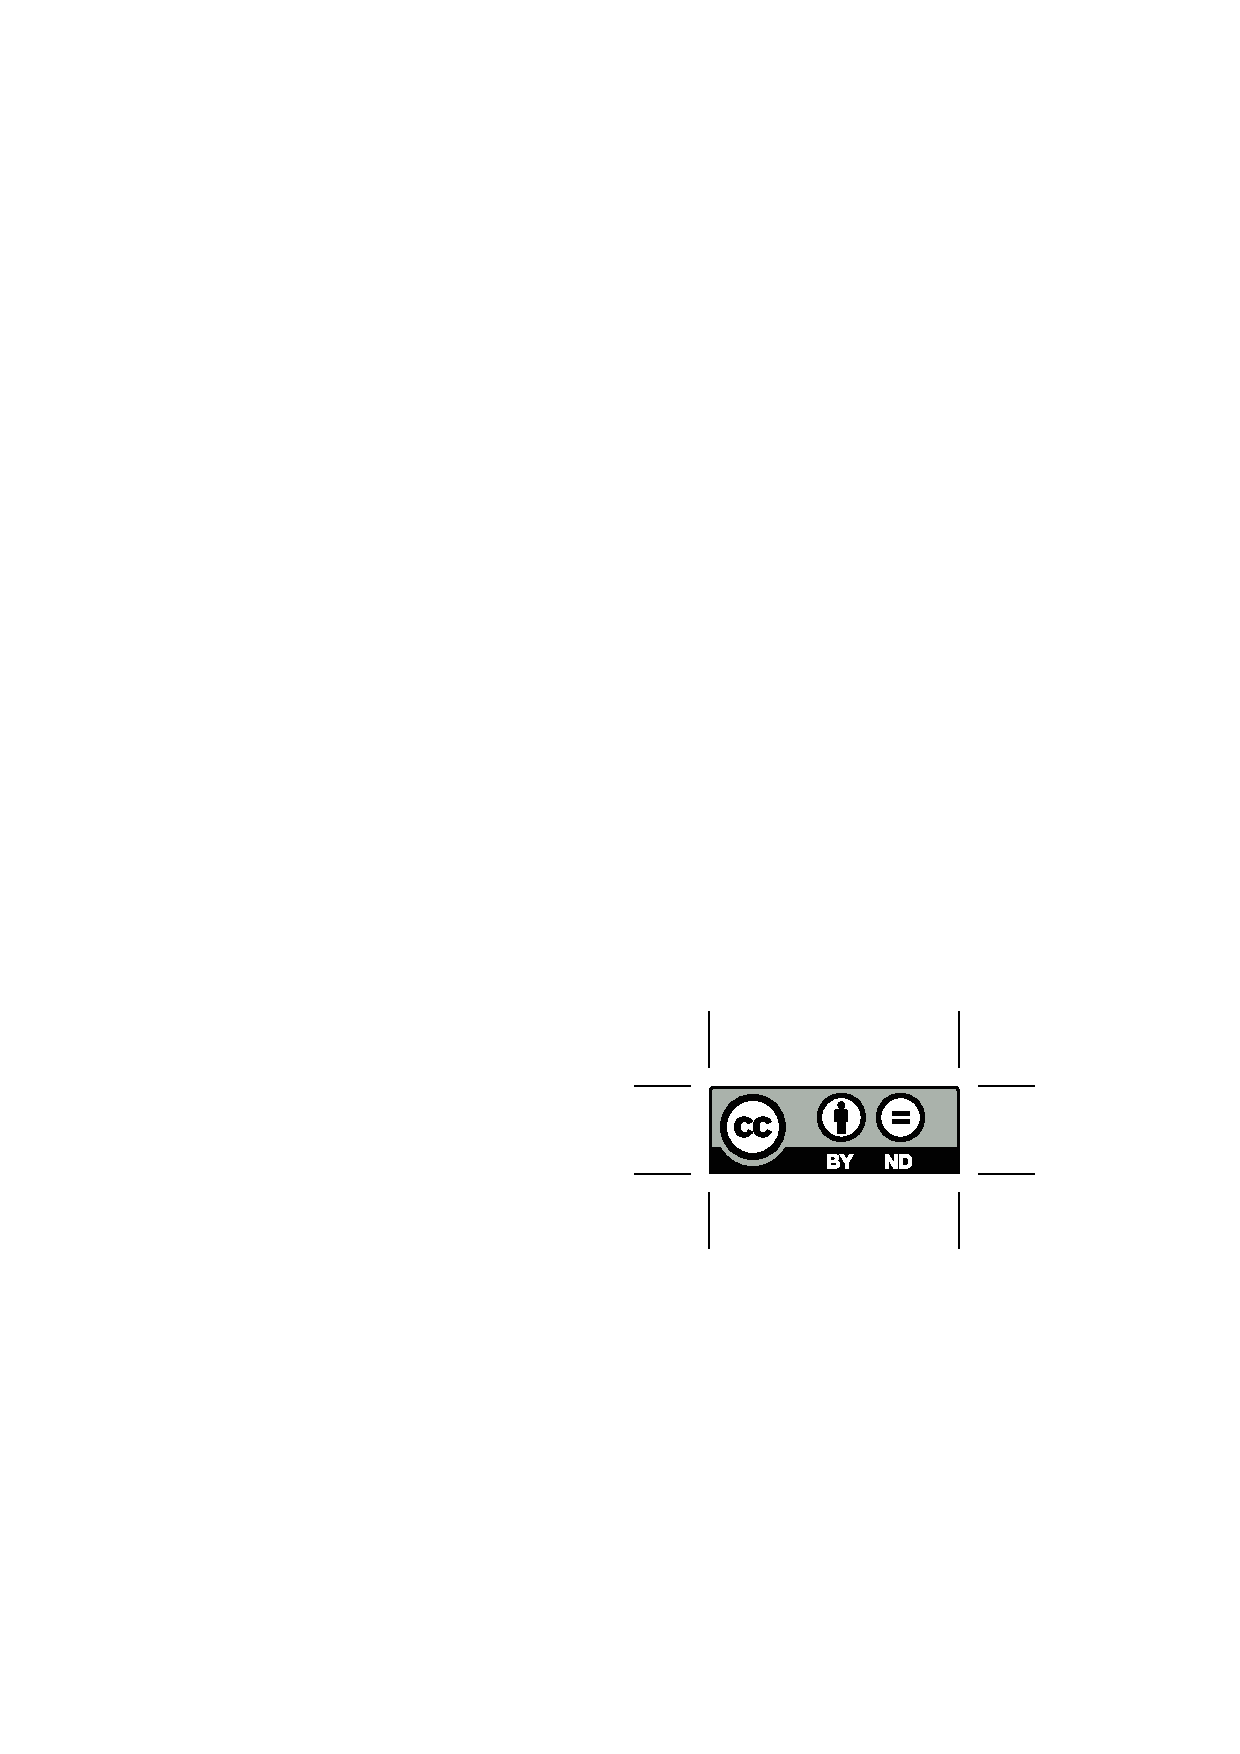
\includegraphics[width=0.5\linewidth]{images/licenses/by-nd}
   \caption{Otra figura.}
   \label{fig:other}
\end{figure}

\lipsum[3]

\section{Segunda sección de otro capítulo}

\noindent \lipsum[4-5]




%%%%%%%%%%%%%%%%%%%%%%%%%%%%%%%%%%%%%%%%%%%%%%%%%%%%%%%%%%%%%%%%%%%%%%%%%%%%%%%
\chapter{Título del Capítulo 3}
\label{chapter:tres}

\chapter{Título del Capítulo 3}
\label{ch:tres}

\noindent Los capítulos intermedios servirán para cubrir los siguientes aspectos: antecedentes, problemática o estado del arte, objetivos, fases y desarrollo del proyecto.

Bla, Bla, Bla, .....

\section{Primera sección de este capítulo}
\section{Segundo apartado de este capítulo}
\section{Tercer apartado de este capítulo}

%%%%%%%%%%%%%%%%%%%%%%%%%%%%%%%%%%%%%%%%%%%%%%%%%%%%%%%%%
\chapter{Título del Capítulo 4}
\label{chapter:cuatro}

\chapter{Título del Capítulo 4}
\label{ch:cuatro}

\noindent Los capítulos intermedios servirán para cubrir los siguientes aspectos: antecedentes, problemática o estado del arte, objetivos, fases y desarrollo del proyecto.

El \autoref{ch:intro} se describió bla, bla, bla …

%%%%%%%%%%%%%%%%%%%%%%%%%%%%%%%%%%%%%%%%%%%%%%%%%%%%%%%%%
\chapter{Conclusiones y líneas futuras}
\label{chapter:Resultados}

\chapter{Conclusiones y líneas futuras}
\label{ch:conclusiones}

\noindent Este capítulo es obligatorio. Toda memoria de Trabajo de Fin de Grado debe incluir unas conclusiones y unas líneas de trabajo futuro 

%%%%%%%%%%%%%%%%%%%%%%%%%%%%%%%%%%%%%%%%%%%%%%%%%%%%%%%%%
\chapter{Summary and Conclusions}
\label{chapter:Conclusiones}

This chapter is compulsory. The memory should include an extended summary and conclusions in english. 

%%%%%%%%%%%%%%%%%%%%%%%%%%%%%%%%%%%%%%%%%%%%%%%%%%%%%%%%%
\chapter{Presupuesto}
\label{chapter:presupuesto}

\chapter{Presupuesto}
\label{ch:presupuesto}

\noindent Este capítulo es obligatorio. Toda memoria de Trabajo de Fin de Grado debe incluir un presupuesto.

\section{Sección Uno}

\begin{table}[htb]
    \begin{center}
        \begin{tabularx}{0.8\textwidth} { X X }
            \toprule
            \textbf{Tipos} & \textbf{Descripción} \\
            \midrule
            AAAA  & BBBB \\
            CCCC  & DDDD \\
            EEEE  & FFFF \\
            GGGG  & HHHH \\
            \bottomrule
        \end{tabularx}
    \end{center}
    \caption{Resumen de tipos}
    \label{tbl:presupuesto}
\end{table}

%%%%%%%%%%%%%%%%%%%%%%%%%%%%%%%%%%%%%%%%%%%%%%%%%%%%%%%%%
\appendix

\chapter{Título del Apéndice 1}
\label{appendix:1}
\section{Algoritmo XXX}
\label{Apendice1:XXX}

\begin{center}
\begin{footnotesize}
\begin{verbatim}

/***********************************************************************************
*
* Fichero .h
*
***********************************************************************************
*
* AUTORES
*   
*
* FECHA
*   
*
* DESCRIPCION
*   
*
************************************************************************************/

\end{verbatim}
\end{footnotesize}
\end{center}

\section{Algoritmo YYY}
\label{Apendice1:YYY}

\begin{center}
\begin{footnotesize}
\begin{verbatim}


/***********************************************************************************
 *
 * Fichero .h
 *
 ***********************************************************************************
 *
 * AUTORES
 *
 * FECHA
 *
 * DESCRIPCION
 *
 *
 ************************************************************************************/
 
\end{verbatim}
\end{footnotesize}
\end{center}

\section{Algoritmo ZZZ}
\label{Apendice1:ZZZ}

\begin{center}
\begin{footnotesize}
\begin{verbatim}


/***********************************************************************************
 *
 * Fichero .h
 *
 ***********************************************************************************
 *
 * AUTORES
 *
 * FECHA
 *
 * DESCRIPCION
 *
 *
 ************************************************************************************/
 
\end{verbatim}
\end{footnotesize}
\end{center}



\chapter{Título del Apéndice 2}
\label{appendix:2}
\chapter{Título del Apéndice 2}
\label{appendix:2}

\section{Otro apéndice: Sección 1}
\lipsum[1]

\section{Otro apéndice: Sección 2}
\lipsum[2]

%%%%%%%%%%%%%%%%%%%%%%%%%%%%%%%%%%%%%%%%%%%%%%%%%%%%%%%%%%
\backmatter
% Aquí figurará la bibliografía
\bibliography{memtfg}
%%%%%%%%%%%%%%%%%%%%%%%%%%%%%%%%%%%%%%%%%%%%%%%%%%%%%%%%%%

\end{document}

